\section{Getting Started}

\subsection{Operating Systems}

Since jModelTest is a Java application, it can be used in every OS that can execute a Java Runtime Environment (JRE). The most common Operating Systems and many other include a JRE (OpenJDK, Sun JRE, ...), or at least it is possible to download one. However, jModelTest depends on third-party binaries (PhyML), that are distributed for Windows, Linux and OsX, and it is even possible to download PhyML sources (http://code.google.com/p/phyml) and compile them for a particular architecture.

\subsection{Working with the repository}

This tool is distributed under GPL v3 license. The source code is freely available at google code repository. You can checkout the repository at \url{http://code.google.com/p/jmodeltest2/source}.

\subsection{User interfaces}

jModelTest can be executed from two different user interfaces, GUI or Console. The Graphical User Interface (GUI) is intended for execution on common desktop computers with multicore processors -most users will probably use this. On the other hand, HPC environments, like multicore clusters, require a non-interactive processing (batch processes), so jModelTest has to be executed from the Command Console Interface. Results are given in plain text format, but an html log is also created.

\subsubsection{Graphical User Interface}

\begin{enumerate}
\item Execute the script for the Graphical User Interface (runjmodeltest-gui.sh). The main jModelTest frame should pop up on the screen:

\begin{center}
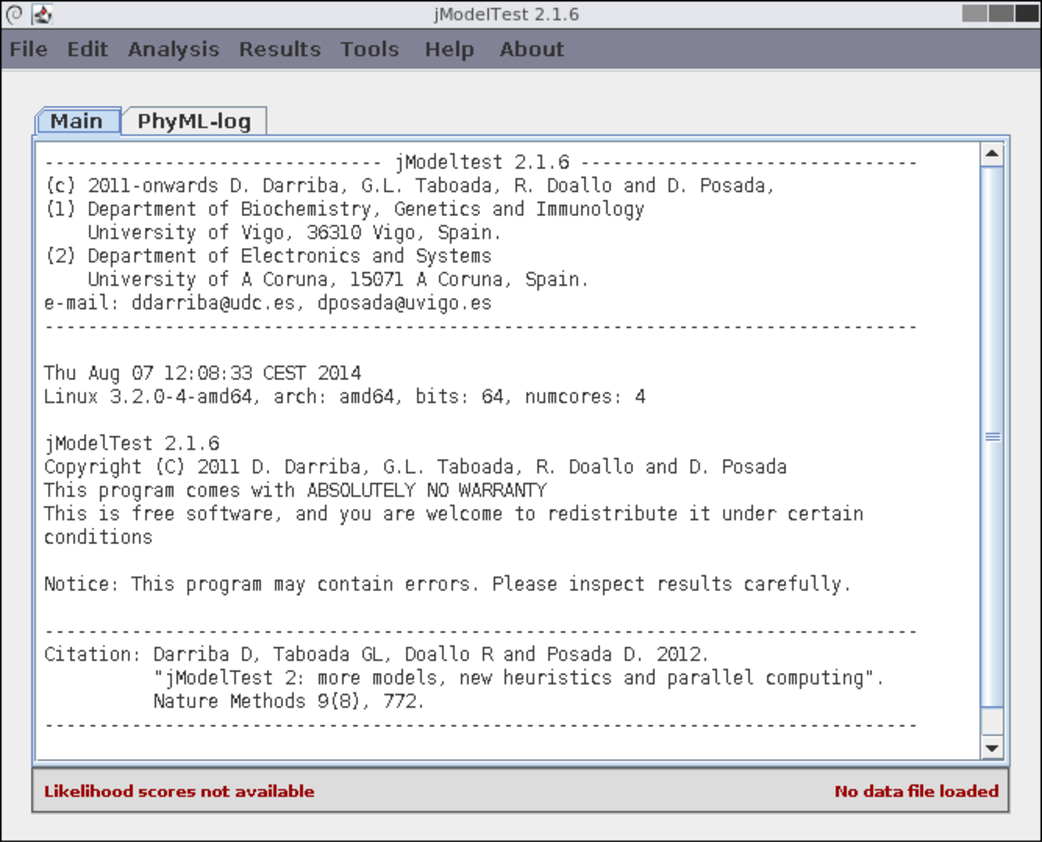
\includegraphics[width=.9\textwidth]{images/main-window}
\end{center}

\item Load an input alignment file using the {\bf File/Load Alignment} option.

\item Go to {\bf Analysis/Compute Likelihood Scores} and select the candidate models and the options for model optimization (optionally you can set a base topology from a file). Press Enter or the {\bf Compute Likelihoods} button.

\begin{center}
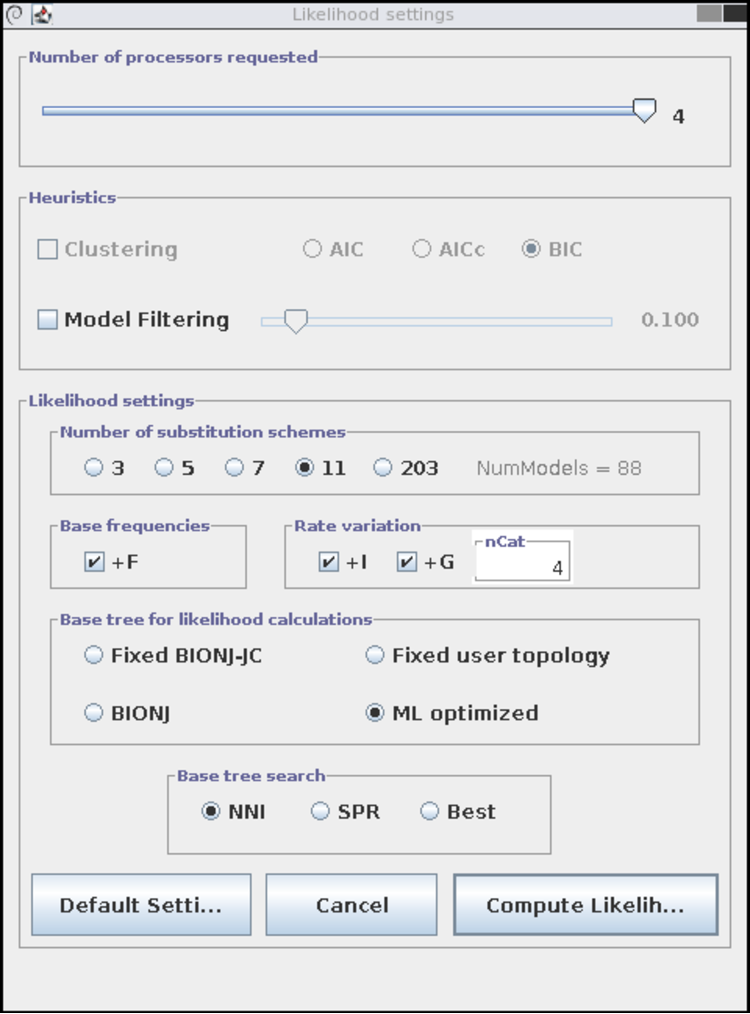
\includegraphics[width=.6\textwidth]{images/lkl-settings}
\end{center}

\item Perform statistical selection among the optimized models. For example, we can calculate the Bayesian Information Criterion using {\bf Analysis/Do BIC calculations...} option, or any other. You can find a Criteria comparison in terms of accuracy in the \href{http://www.nature.com/nmeth/journal/v9/n8/extref/nmeth.2109-S1.pdf}{supplementary material} of the \href{http://www.nature.com/nmeth/journal/v9/n8/full/nmeth.2109.html}{jModelTest publication}.

\begin{center}
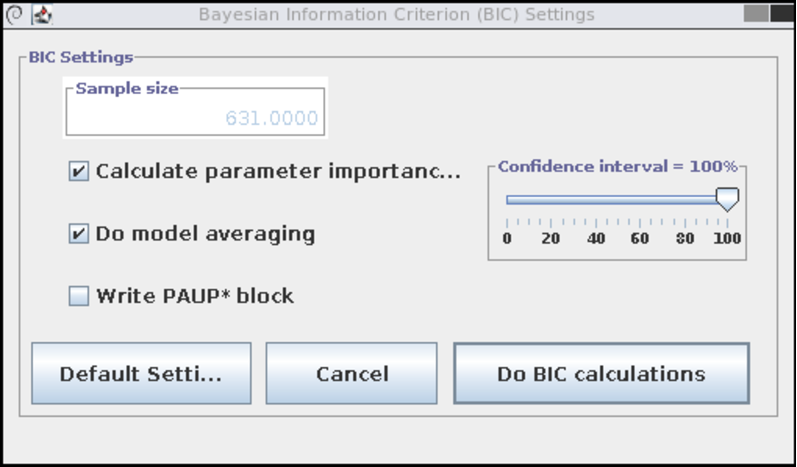
\includegraphics[width=.6\textwidth]{images/bic}
\end{center}

The results will be shown in the main console.

\item Take a look at the results table in {\bf Results/Show results table}. Best model is the one with the lowest criterion value (BIC column in the example) and therefore delta = 0.

\begin{center}
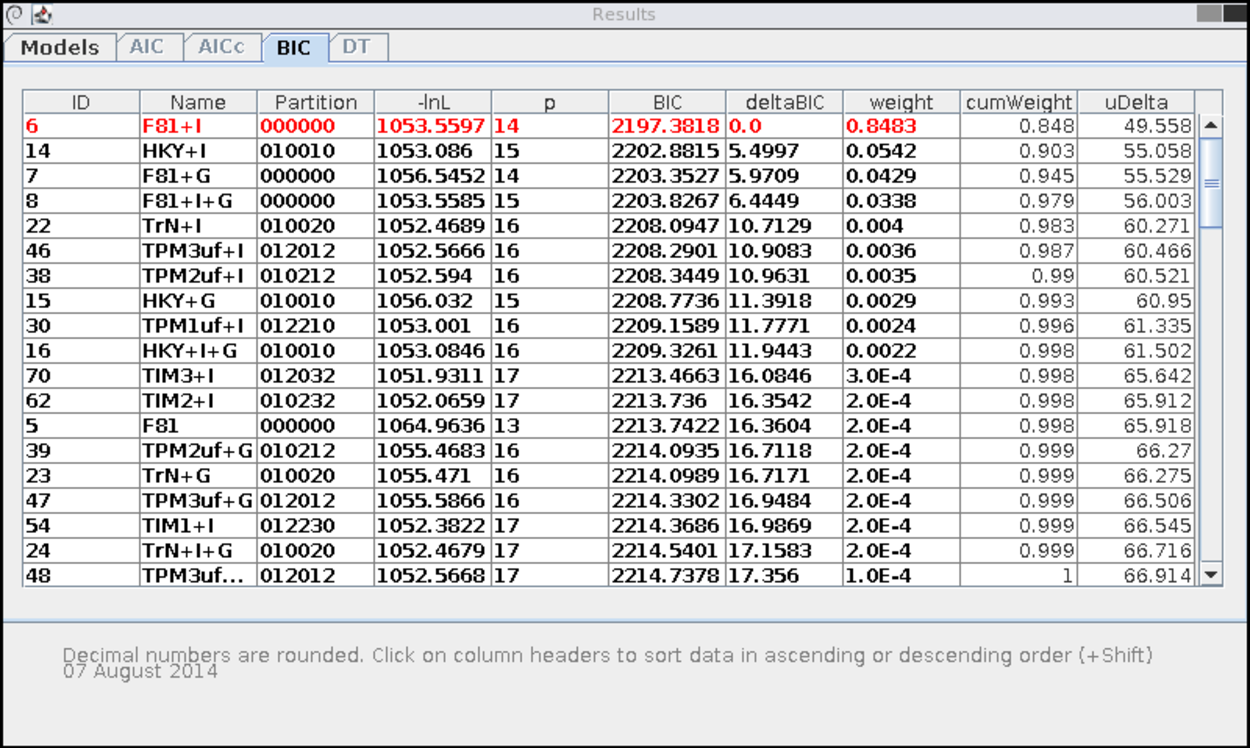
\includegraphics[width=.9\textwidth]{images/results}
\end{center}

\item Build a consensus tree from a given selection criteria using {\bf Analysis/Model-averaged phylogeny}:

\begin{center}
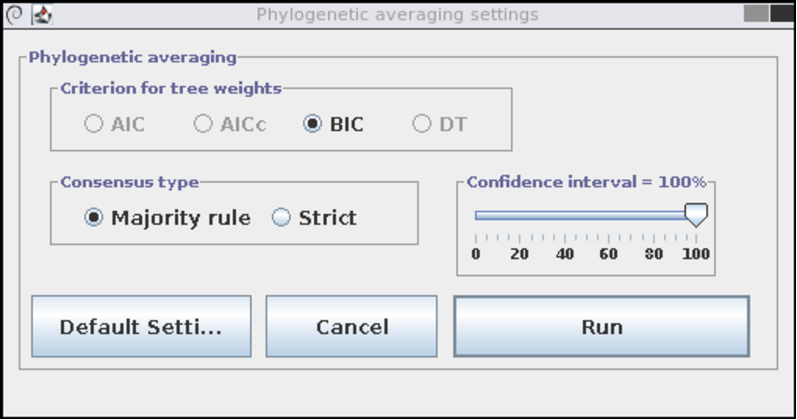
\includegraphics[width=.6\textwidth]{images/consensus}
\end{center}

\item Finally, you can save the results displayed in the main console using {\bf Edit/Save console}. Alternatively, you can get a formatted HTML document using {\bf Results/Build HTML log}:

\begin{center}
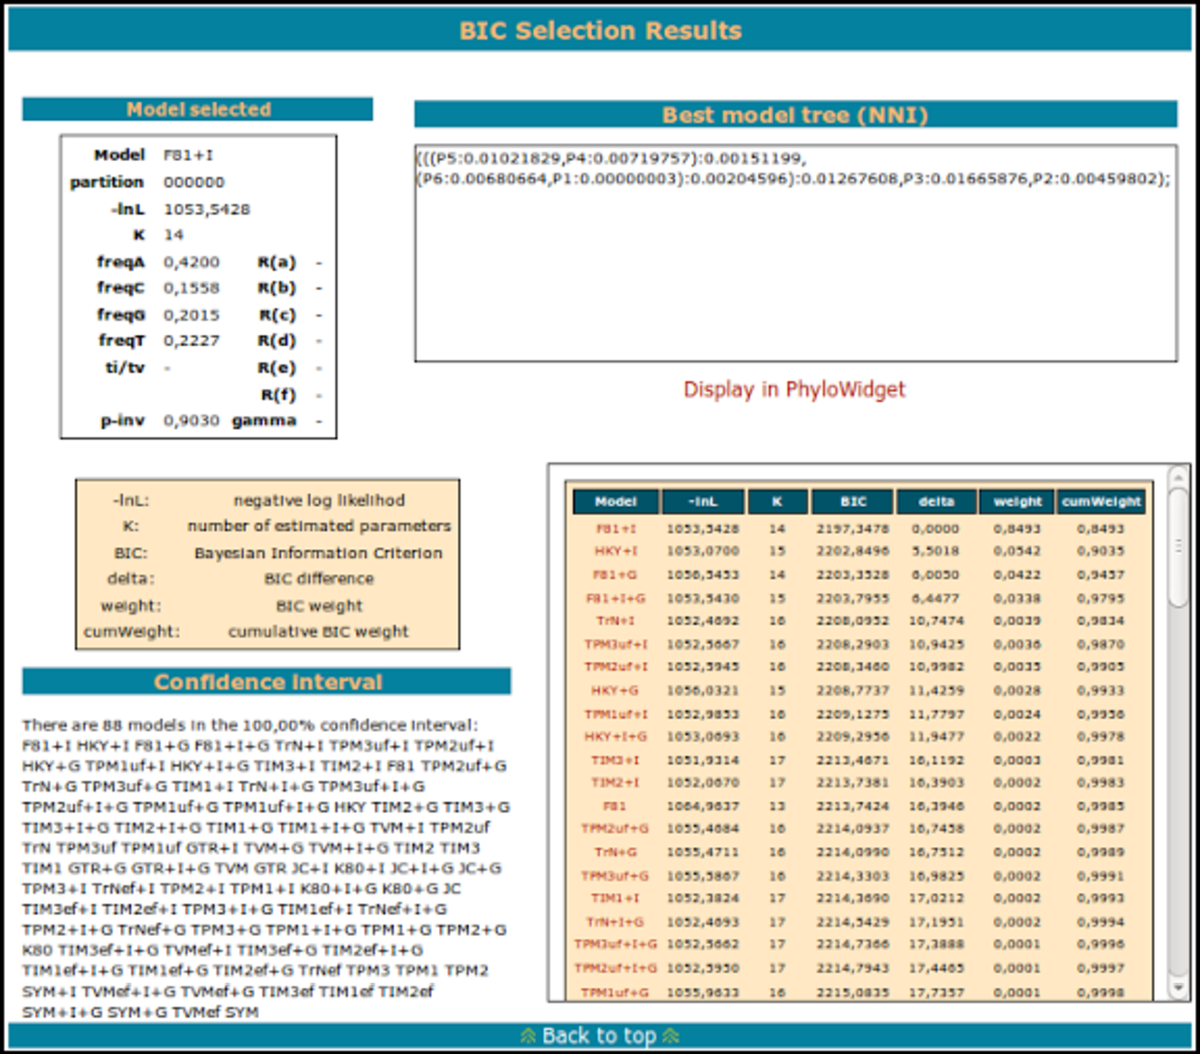
\includegraphics[width=.9\textwidth]{images/html-log}
\end{center}

Take a look at Section \ref{sec:gui} for further information.

\end{enumerate}

\subsubsection{Command Console Interface}

\begin{enumerate}
\item Execute the following command line:
\begin{lstlisting}
$ java -jar jModelTest.jar -d example-data/aP6.fas -g 4 -i -f -AIC -BIC -a
\end{lstlisting}

This will test all 88 models (gamma models with 4 rate categories), and then perform the model selection using Akaike (AIC) and Bayesian (BIC) criteria, calculating also a model averaged phylogeny (-a).

See Section~\ref{sec:arguments} for information about supported arguments.

\item This will generate the following output:

\begin{enumerate}

\item Header:

\begin{lstlisting}
----------------------------- jModeltest 2.0 -----------------------------
(c) 2011-onwards Diego Darriba, David Posada,
Department of Biochemistry, Genetics and Immunology
University of Vigo, 36310 Vigo, Spain. e-mail: ddarriba@udc.es, dposada@uvigo.es
--------------------------------------------------------------------------------
Wed Oct 05 12:56:47 CEST 2011
Linux 2.6.38-11-generic-pae, arch: i386, bits: 32, numcores: 2

jModelTest 2.0  Copyright (C) 2011 Diego Darriba, David Posada
This program comes with ABSOLUTELY NO WARRANTY
This is free software, and you are welcome to redistribute it
under certain conditions
 
Notice: This program may contain errors. Please inspect results carefully.
\end{lstlisting}

\item Execution options:

\begin{lstlisting} 
Arguments = -d example-data/aP6.fas -g 4 -i -f -AIC -BIC -a

Reading data file "aP6.fas"... OK.
  number of sequences: 6
  number of sites: 631
 
 
---------------------------------------------------------------
*                                                             *
*        COMPUTATION OF LIKELIHOOD SCORES WITH PHYML          *
*                                                             *
---------------------------------------------------------------
 
::Settings::
 Phyml version = 3.0
 Phyml binary = PhyML_3.0_linux32
 Candidate models = 24
  number of substitution schemes = 3
  including models with equal/unequal base frequencies (+F)
  including models with/without a proportion of invariable sites (+I)
  including models with/without rate variation among sites (+G) (nCat = 4)
 Optimized free parameters (K) = substitution parameters + 9 branch lengths + topology 
 Base tree for likelihood calculations = ML tree
 Tree topology search operation = NNI
computing likelihood scores for 24 models with Phyml 3.0
\end{lstlisting}

\item Real time optimization results (progress):

\begin{lstlisting}
::Progress::

Model 		 Exec. Time 	 Total Time 	 -lnL
-------------------------------------------------------------------------
JC		00h:00:00:01	00h:00:00:01	1114,9772
JC+G		00h:00:00:04	00h:00:00:05	1106,4431
...
GTR+G		00h:00:00:06	00h:00:06:07	1054,7203
GTR+I+G		00h:00:01:02	00h:00:07:05	1051,8403
\end{lstlisting}

\item Sorted and complete optimization results:

\begin{lstlisting}
   Model = JC
   partition = 000000
   -lnL = 1114.9772
   K = 10 
 
   Model = JC+I
   partition = 000000
   -lnL = 1103.1113
   K = 11
   p-inv = 0.9080 

...

   Model = GTR+I+G
   partition = 012345
   -lnL = 1051.8403
   K = 20
   freqA = 0.4235 
   freqC = 0.1520 
   freqG = 0.2022 
   freqT = 0.2224 
   R(a) [AC] =  0.8709
   R(b) [AG] =  0.4152
   R(c) [AT] =  0.6049
   R(d) [CG] =  1.2523
   R(e) [CT] =  0.9482
   R(f) [GT] =  1.0000
   p-inv = 0.5940
   gamma shape = 0.0120 
 
 
Computation of likelihood scores completed. It took 00h:00:07:05.
\end{lstlisting}

\item Selected Information Criteria (best model and all models sorted according to each criterion):

\begin{lstlisting}
---------------------------------------------------------------
*                                                             *
*             AKAIKE INFORMATION CRITERION (AIC)              *
*                                                             *
---------------------------------------------------------------
 
 Model selected: 
   Model = F81+I
   partition = 000000
   -lnL = 1053.5428
   K = 14
   freqA = 0.4200 
   freqC = 0.1558 
   freqG = 0.2015 
   freqT = 0.2227 
   p-inv = 0.9030 
 
ML tree (NNI) for the best AIC model = (((P5:0.01021829,P4:0.00719757):0.00151199,(P6:0.00680664,P1:0.00000003):0.00204596):0.01267608,P3:0.01665876,P2:0.00459802);
 
 
* AIC MODEL SELECTION : Selection uncertainty
 
Model             -lnL    K         AIC      delta      weight cumWeight
------------------------------------------------------------------------ 
F81+I        1053.5428   14   2135.0855     0.0000      0.4332    0.4332 
HKY+I        1053.0700   15   2136.1401     1.0545      0.2557    0.6890 
F81+I+G      1053.5430   15   2137.0859     2.0004      0.1594    0.8483
...
K80          1114.5049   11   2251.0098   115.9243   2.91e-026    1.0000 
SYM          1114.4117   15   2258.8235   123.7380   5.85e-028    1.0000
------------------------------------------------------------------------
-lnL:	negative log likelihod
 K:	number of estimated parameters
 AIC:	Akaike Information Criterion
 delta:	AIC difference
 weight:	AIC weight
 cumWeight:	cumulative AIC weight
 
 
* AIC MODEL SELECTION : Confidence interval
 
There are 24 models in the 100% confidence interval: [ F81+I HKY+I F81+I+G HKY+I+G F81+G GTR+I HKY+G GTR+I+G GTR+G F81 HKY GTR JC+I K80+I JC+I+G K80+I+G JC+G K80+G SYM+I SYM+I+G SYM+G JC K80 SYM ] 
\end{lstlisting}

\item Consensus tree of the optimized phylogenies using the criterion weights:
 
\begin{lstlisting}
---------------------------------------------------------------
*                                                             *
*                    MODEL AVERAGED PHYLOGENY                 *
*                                                             *
---------------------------------------------------------------
 
Selection criterion: . . . . AIC
Confidence interval: . . . . 1.00
Consensus type:. . . . . . . 50% majority rule
 
 
Using 24 models in the 1.00 confidence interval = F81+I HKY+I F81+I+G HKY+I+G F81+G GTR+I HKY+G GTR+I+G GTR+G F81 HKY GTR JC+I K80+I JC+I+G K80+I+G JC+G K80+G SYM+I SYM+I+G SYM+G JC K80 SYM  

Bipartitions included in the consensus tree
 
    123456
    ****** ( 1.0 )
    ****-- ( 1.0 )
    **---- ( 0.94244 )
    --**-- ( 1.0 )

 
                        +-----------6 P4
                      +-8
                      | +----------------5 P5
+---------------------9
|                     |  +-4 P1
|                     +--7
|                        +----------3 P6
|
+------2 P2
|
+---------------------------1 P3

 
(P3:0.016613,P2:0.004598,((P6:0.006790,P1:0.000000)1.00:0.002046,(P5:0.010191,P4:0.007198)0.94:0.001510)1.00:0.012665);
 
Note: this tree is unrooted. Branch lengths are the expected number of substitutions per site. Labels next to parentheses represent phylogenetic uncertainty due to model selection (see documentation)
\end{lstlisting}

\item Also a HTML log is automatically stored in the ``log'' directory.

\end{enumerate}
\end{enumerate}

\subsection{High Performance Environments}

\subsubsection{Shared memory architectures (multicore systems)}

Both the GUI and Console interfaces can be used for shared memory architectures. See Graphical User Interface or Command Console Interface. In some dedicated HPC environments you can only use the console interface, for example when using a bath-queuing system like Oracle Grid Engine. Additionally, in the console version you can specify the number of threads you want to use using the -tr'' option. By default, the total number of cores in the machine is used.

\subsubsection{Distributed memory architectures (HPC clusters)}

\begin{enumerate}
\item Besides the multithreading support, it is possible to run jModelTest in a cluster. This feature has been implemented using a Java message-passing (MPJ) library, MPJ Express (http://mpj-express.org/). To execute jModelTest in a cluster environment you have to:

\begin{lstlisting}
$ export $JMODELTEST_HOME=[path_to_jModelTest]
$ cd $JMODELTEST_HOME
$ tar zvxf mpj.tar.gz
$ export MPJ_HOME=$JMODELTEST_HOME/mpj
$ export PATH=$MPJ_HOME/bin:$PATH
$ cp $JMODELTEST_HOME/extra/machines $JMODELTEST_HOME
\end{lstlisting}

You can also add the last two lines to ~/.bashrc to automatically set these variables at console startup.

\item \$JMODELTEST\_HOME/machines file contains the set of computing nodes where the mpj processes will be executed. By default it points to the localhost machine, so you should change it if you want to run a parallel execution over a cluster machine, just writing on each line the particular computing nodes (e.g. see filecluster8.conf.template).

\item Start the MPJ Express daemons:

\begin{lstlisting}
$ mpjboot machines
\end{lstlisting}

The application ``mpjboot'' should be in the execution path (it is located at \$MPJ\_HOME/bin). A ssh service must be running in the machines listed in the machines file. Moreover, port 10000 should be free. For more details refer to the MPJ Express documentation.

\item Run jModelTest. For this, the jModelTest distribution provides a bash script: 'runjmodeltest-cluster.sh'

The basic syntax is:

./runjmodeltest-cluster.sh \$NUMBER\_OF\_PROCESSORS \$APPLICATION\_PARAMETERS

\begin{lstlisting}
$ ./runjmodeltest-cluster.sh 2 -d example-data/aP6.fas -s 11 -i -g 4 -f -AIC -a
\end{lstlisting}

\end{enumerate}
